\documentclass[UTF8,11pt]{ctexart}
\usepackage[a4paper,margin=22mm]{geometry}
\usepackage{graphicx,enumitem,amssymb,tabularx}
\usepackage[normalem]{ulem}
\usepackage{xeCJKfntef}
\setlength{\parindent}{0pt}
\setlength{\parskip}{.6em}
\sloppy
\begin{document}
\section*{2014年12月英语六级真题(第2套)}
\subsection*{2014 年12 月大学英语六级考试真题(二）}


\subsection*{\textbf{Part I} \textbf{Writing} \textbf{(30 minutes)}}


Directions：\textit{For this part, you are allowed 30 minutes to write an essay based on the picture below. You should start your} \textit{essay with a brief description of the picture and then discuss whether there is a shortcut to learning. You should give sound}


\subsection*{\textit{arguments to support your views and write at least}\textbf{\textit{ }}\textbf{\textit{\uline{150}}}\textit{ words but no more than 200 words}.}


\begin{center}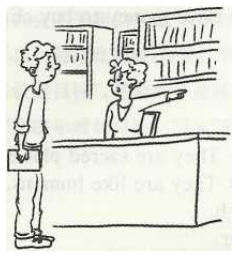
\includegraphics[width=.85\linewidth,height=.55\textheight,keepaspectratio]{2014-12-02.assets/figure-001-004.png}\end{center}

“‘How To Do Well In School Without Studying’ is over there in the fiction section.”


注意：此部分试题请在答题卡1 上作答。


\textbf{Part}II \textbf{Listening Comprehension} \textbf{(30 minutes)}


\subsection*{\textbf{Section A}}


\textbf{Directions}：\textit{In this section},\textit{ you will hear 8 short conversations and 2 long conversations. At the end of each conversation}, \textit{one or more questions will be asked about what was said}.\textit{ Both the conversation and the questions will be spoken only once.} \textit{After each question there will be a pause}.\textit{ During the pause}，\textit{you must read the four choices marked A) 9 B) 9} C)\textit{ and D)} ,\textit{ and}


\subsection*{\textit{decide which is the best answer. Then mark the corresponding letter on}\textbf{\textit{ Answer Sheet 1}}\textit{ with a single line through the}}


\textit{centre}. 注意：此部分试题请在答题卡1 上作答。


\noindent\begin{tabularx}{\linewidth}{@{}lXXXX@{}}1. & \textbf{A.} In a parking lot. & \textbf{B.} At a grocery. & \textbf{C.} At a fast food restaurant. & \textbf{D.} In a car showroom.\\\end{tabularx}\par

2.


\begin{itemize}[leftmargin=2em,itemsep=.2em,topsep=.4em]\item[A.] Change her position now and then.
\item[B.] Stretch her legs before standing up.
\item[C.] Have a little nap after lunch.
\item[D.] Get up and take a short walk.
\end{itemize}

3.


\begin{itemize}[leftmargin=2em,itemsep=.2em,topsep=.4em]\item[A.] The students should practice long-distance running.
\item[B.] The students’ physical condition is not desirable.
\item[C.] He doesn’t quite believe what the woman says.
\item[D.] He thinks the race is too hard for the students.
\end{itemize}

4.


\begin{itemize}[leftmargin=2em,itemsep=.2em,topsep=.4em]\item[A.] They will get their degrees in two years.
\item[B.] They are both pursuing graduate studies.
\item[C.] They cannot afford to get married right now.
\item[D.] They do not want to have a baby at present.
\end{itemize}

5.


\begin{itemize}[leftmargin=2em,itemsep=.2em,topsep=.4em]\item[A.] He must have been mistaken for Jack.
\item[B.] Twins usually have a lot in common.
\item[C.] Jack is certainly not as healthy as he is.
\item[D.] He has not seen Jack for quite a few days.
\end{itemize}

6.


\begin{itemize}[leftmargin=2em,itemsep=.2em,topsep=.4em]\item[A.] The woman will attend the opening of the museum.
\item[B.] The woman is asking the way at the crossroads.
\item[C.] The man knows where the museum is located.
\item[D.] The man will take the woman to the museum.
\end{itemize}

7.


\begin{itemize}[leftmargin=2em,itemsep=.2em,topsep=.4em]\item[A.] They cannot ask the guy to leave.
\item[B.] The guy has been coming in for years.
\item[C.] The guy must be feeling extremely lonely.
\item[D.] They should not look down upon the guy.
\end{itemize}

1


8.


\begin{itemize}[leftmargin=2em,itemsep=.2em,topsep=.4em]\item[A.] Collect timepieces.
\item[B.] Become time-conscious.
\item[C.] Learn to mend clocks.
\item[D.] Keep track of his daily activities.
\end{itemize}

\textbf{Questions 9 to 11 are based on the conversation you have just heard.}


9.


\begin{itemize}[leftmargin=2em,itemsep=.2em,topsep=.4em]\item[A.] It is eating into its banks.
\item[B.] It winds its way to the sea.
\item[C.] It is wide and deep.
\item[D.] It is quickly rising.
\end{itemize}

10.


\begin{itemize}[leftmargin=2em,itemsep=.2em,topsep=.4em]\item[A.] Try to speed up the operation by any means.
\item[B.] Take the equipment apart before being ferried.
\item[C.] Reduce the transport cost as much as possible.
\item[D.] Get the trucks over to the other side of the river.
\end{itemize}

11.


\begin{itemize}[leftmargin=2em,itemsep=.2em,topsep=.4em]\item[A.] Find as many boats as possible.
\item[B.] Cut trees and build rowing boats.
\item[C.] Halt the operation until further orders.
\item[D.] Ask the commander to send a helicopter.
\end{itemize}

\textbf{Questions 12 to 15 are based on the conversation you have just heard.}


12.


\begin{itemize}[leftmargin=2em,itemsep=.2em,topsep=.4em]\item[A.] Talk about his climbing experiences.
\item[B.] Help him join an Indian expedition.
\item[C.] Give up mountain climbing altogether.
\item[D.] Save money to buy climbing equipment.
\end{itemize}

13.


\begin{itemize}[leftmargin=2em,itemsep=.2em,topsep=.4em]\item[A.] He was the first to conquer Mt. Qomolangma.
\item[B.] He had an unusual religious background.
\item[C.] He climbed mountains to earn a living.
\item[D.] He was very strict with his children.
\end{itemize}

\noindent\begin{tabularx}{\linewidth}{@{}lXXXX@{}}14. & \textbf{A.} They are to be conquered. & \textbf{B.} They are to be protected. & \textbf{C.} They are sacred places. & \textbf{D.} They are like humans.\\\end{tabularx}\par

15.


\begin{itemize}[leftmargin=2em,itemsep=.2em,topsep=.4em]\item[A.] It was his father’s training that pulled him through.
\item[B.] It was a milestone in his mountain climbing career.
\item[C.] It helped him understand the Sherpa view of mountains.
\item[D.] It was his father who gave him the strength to succeed.
\end{itemize}

\subsection*{\textbf{Section B}}


\textbf{Directions}：\textit{In this section, you will hear 3 short passages. At the end of each passage, you will hear some questions. Both} \textit{the passage and the questions will be spoken only once. After you hear a question},\textit{ you must choose the best answer from the}


\subsection*{\textit{four choices marked A}) ,\textit{ B)},\textit{ C})\textit{ and D). Then mark the corresponding letter on} \textbf{\textit{Answer Sheet 1}}\textit{ with a single line through}}


\textit{the centre}. 注意：此部分试题请在答题卡1 上作答6\textbf{Passage} \textbf{One}


\textbf{Questions 16 to 19 are based on the passage you have just heard.}


16.


\begin{itemize}[leftmargin=2em,itemsep=.2em,topsep=.4em]\item[A.] By showing a memorandum’s structure.
\item[B.] By analyzing the organization of a letter.
\item[C.] By comparing memorandums with letters.
\item[D.] By reviewing what he has said previously.
\end{itemize}

17.


\begin{itemize}[leftmargin=2em,itemsep=.2em,topsep=.4em]\item[A.] They ignored many of the memorandums they received.
\item[B.] They placed emphasis on the format of memorandums.
\item[C.] They seldom read a memorandum through to the end.
\item[D.] They spent a lot of time writing memorandums.
\end{itemize}

\noindent\begin{tabularx}{\linewidth}{@{}lXXXX@{}}18. & \textbf{A.} Style and wording. & \textbf{B.} Directness and clarity. & \textbf{C.} Structure and length. & \textbf{D.} Simplicity and accuracy.\\\end{tabularx}\par

19.


\begin{itemize}[leftmargin=2em,itemsep=.2em,topsep=.4em]\item[A.] Inclusion of appropriate humor.
\item[B.] Direct statement of purpose.
\item[C.] Professional look.
\item[D.] Accurate dating.
\end{itemize}

\subsection*{\textbf{Passage Two}}


\textbf{Questions 20 to 22 are based on the passage you have just heard.}


20.


\begin{itemize}[leftmargin=2em,itemsep=.2em,topsep=.4em]\item[A.] They give top priority to their work efficiency.
\item[B.] They make an effort to lighten their workload.
\end{itemize}

2


\begin{itemize}[leftmargin=2em,itemsep=.2em,topsep=.4em]\item[C.] They try hard to make the best use of their time.
\item[D.] They never change work habits unless forced to.
\end{itemize}

\noindent\begin{tabularx}{\linewidth}{@{}lXXXX@{}}21. & \textbf{A.} Sense of duty. & \textbf{B.} Self-confidence. & \textbf{C.} Work efficiency. & \textbf{D.} Passion for work.\\\end{tabularx}\par

22.


\begin{itemize}[leftmargin=2em,itemsep=.2em,topsep=.4em]\item[A.] They find no pleasure in the work they do.
\item[B.] They try to avoid work whenever possible.
\item[C.] They are addicted to playing online games.
\item[D.] They simply have no sense of responsibility.
\end{itemize}

\subsection*{\textbf{Passage Three}}


\textbf{Questions 23 to 25 are based on the passage you have just heard.}


23.


\begin{itemize}[leftmargin=2em,itemsep=.2em,topsep=.4em]\item[A.] He lost all his property.
\item[B.] He was sold to a circus.
\item[C.] He ran away from his family.
\item[D.] He was forced into slavery.
\end{itemize}

\noindent\begin{tabularx}{\linewidth}{@{}lXXXX@{}}24. & \textbf{A.} A carpenter. & \textbf{B.} A master of his. & \textbf{C.} A businessman. & \textbf{D.} A black drummer.\\\end{tabularx}\par

25.


\begin{itemize}[leftmargin=2em,itemsep=.2em,topsep=.4em]\item[A.] It named its town hall after Solomon Northup.
\item[B.] It freed all blacks in the town from slavery.
\item[C.] It declared July 24 Solomon Northup Day.
\item[D.] It hosted a reunion for the Northup family.
\end{itemize}

\subsection*{\textbf{Section C}}


\textbf{Directions}：\textit{In this section, you will hear a passage three times. When the passage is read for the first time},\textit{ you should listen} \textit{carefully for its general idea. When the passage is read for the second time},\textit{ you are required to fill in the blanks with the} \textit{exact words you have just heard. Finally, when the passage is read for the third time, you should check what you have} \textit{written.} 注意：此部分试题请在答题卡1 上作答。


Intolerance is the art of ignoring any views that differ from your own. It \uline{26} itself in hatred, stereotypes, prejudice, and \uline{27} Once it intensifies in people, intolerance is nearly impossible to overcome. But why would anyone want to be labeled\textit{ intolerant?} Why would people want to be \uline{28} about the world around them? Why would one want to be part of the problem in America, instead of the solution?


There are many explanations for intolerant attitudes, some \uline{29} childhood. It is likely that intolerant folks grew up\uline{ 30} intolerant parents and the cycle of prejudice has simply continued for\uline{ 31} . Perhaps intolerant people are so set in their ways that they find it easier to ignore anything that might not\uline{ 32 }their limited view of life. Or maybe intolerant students have simply never been \uline{33} to anyone different from themselves. But none of these reasons is an excuse for allowing the intolerance to continue.


Intolerance should not be confused with disagreement. It is, of course, possible to disagree with an opinion without being intolerant of it/If you understand a belief but still don’t believe in that specific belief, that’s fine. You are \uline{34} your opinion. As a matter of fact, \uline{35} \textit{dissenters}(持异议者) are important for any belief. If we all believed the same things, we would never grow? and we would never learn about the world around us. Intolerance does not stem from disagreement. It stems from fear. And fear stems from ignorance.


\textbf{Part}III \textbf{Reading Comprehension} \textbf{(40 minutes)}


\subsection*{\textbf{Section A}}


\textbf{Directions}：\textit{In this section 9 there is a passage with ten blanks. You are required to select one word for each blank from a} \textit{list of choices given in a word bank following the passage}.\textit{ Read the passage through carefully before making your choices.}


\subsection*{\textit{Each choice in the bank is identified by a letter. Please mark the corresponding letter for each item on}\textbf{\textit{ Answer Sheet 2}}}


\textit{with a single line through the centre. You may not use any of the words in the bank more than once}.


\textbf{Questions 36 to 45 are based on the following passage.}


His future subjects have not always treated the Prince of Wales with the respect one might expect. They laughed aloud in 1986 when the heir to the British \uline{36} told a TV reporter that he talked to his plants at his country house, Highgrove, to stimulate


3


their growth. The Prince was being humorous —“My sense of humor will get me into trouble one day,“ he said to his\textit{ aids}（随从） —but listening to Charles Windsor can indeed prove stimulating. The royal \uline{37} has been promoting radical ideas for most of his adult life. Some of his \uline{38} ，which once sounded a bit weird, were simply ahead of their time. Now, finally, the world seems to be catching up with him.


Take his views on farming. Prince Charles’ Duchy Home Farm went \uline{39} back in 1986, when most shoppers cared only about the low price tag on suspiciously\textit{ blemish-free}(无瑕戚的）vegetables and \uline{40} large chickens piled high in supermarkets.


His warnings on climate change proved farsighted, too. Charles began \uline{41} action on global warming in 1990 and says he has been worried about the \uline{42} of man on the environment since he was a teenager.


Although he has gradually gained international \uline{43} as one of the world’s leading conservationists, many British people still think of him as an \uline{44} person who talks to plants. This year, as it happens, South Korean scientists proved that plants really do \uline{45} to sound. So Charles was ahead of the game there, too. 注\CJKunderline{意：此部分试题请在答题卡2 上作答。}


\begin{itemize}[leftmargin=2em,itemsep=.2em,topsep=.4em]\item[A.] conform
\item[B.] eccentric
\item[C.] environmentalist
\item[D.] expeditions
\item[E.] impact
\item[F.] notions
\item[G.] organic
\item[H.] originally
\item[I.] recognition
\item[J.] respond
\item[K.] subordinate
\item[L.] suppressing
\item[M.] throne
\item[N.] unnaturally
\item[O.] urging
\end{itemize}

\subsection*{\textbf{Section B}}


Directions：\textit{In this section, you are going to read a passage with ten statements attached to it. Each statement contains} \textit{information given in one of the paragraphs. Identify the paragraph from which the information is derived. You may choose} \textit{a paragraph more than once. Each paragraph is marked with a letter. Answer the questions by marking the corresponding}


\subsection*{\textit{letter on}\textbf{\textit{ Answer Sheet 2.}}}


High School Sports Aren’t Killing Academics


A) In this months\textit{ Atlantic} cover article, “The Case Against High-School Sports,” Amanda Ripley argues that school-sponsored sports programs should be seriously cut. She writes that, unlike most countries that outperform the United States on international assessments, American schools put too much of an emphasis on athletics. “Sports are embedded in American schools in a way they are not almost anywhere else，” she writes. “Yet this difference hardly ever comes up in domestic debates about America’s international\textit{ mediocrity} (平庸) in education.”


B) American student-athletes reap many benefits from participating in sports, but the costs to the schools could outweigh their benefits, she argues. In particular, Ripley contends that sports crowd out the academic missions of schools：America should learn from South Korea and Finland and every other country at the top level of international test scores, all of whom emphasize athletics far less in school. “Even in eighth grade, American kids spend more than twice the time Korean kids spend playing sports，” she writes, citing a 2010 study published in the\textit{ Journal of Advanced Academics.}


C) It might well be true that sports are far more rooted in American high schools than in other countries. But our reading of international test scores finds no support for the argument against school athletics. Indeed, our own research and that of others lead us to make the opposite case. School-sponsored sports appear to provide benefits that seem to increase, not\textit{ detract} (减少)from, academic success.


D) Ripley indulges a popular\textit{ obsession} (痴迷) with international test score comparisons,which show wide and frightening gaps between the United States and other countries. She ignores, however, the fact that states vary at least as much in test scores as do developed countries. A 2011 report from Harvard University shows that Massachusetts produces math scores comparable to South Korea and Finland, while Mississippi scores are closer to Trinidad and Tobago. Ripley’s thesis about sports falls apart in light of this fact. Schools in Massachusetts provide sports programs while schools in Finland do not. Schools in Mississippi may love football while in Tobago interscholastic sports are nowhere near as prominent. Sports cannot explain


4


these similarities in performance. They can’t explain international differences either.


E) If it is true that sports undermine the academic mission of American schools, we would expect to see a negative relationship between the commitment to athletics and academic achievement. However, the University of Arkansas’s Daniel Bowen and Jay Greene actually find the opposite. They examine this relationship by analyzing schools’ sports winning percentages as well as student-athletic participation rates compared to graduation rates and standardized test score achievement over a five-year period for all public high schools in Ohio. Controlling for student poverty levels,\textit{ demographics}(人口统计4 大况）， and district financial resources, both measures of a school’s commitment to athletics are significantly and positively related to lower dropout rates as well as higher test scores.


F) On-the-field success and high participation in sports is not random —it requires focus and dedication to athletics. One might think this would lead schools obsessed with winning to deemphasize academics. Bowen and Greene’s results contradict that argument. A likely explanation for this seemingly\textit{ counterintuitive} (与直觉相反的）result is that success in sports programs actually facilitates or rejects greater social capital within a school’s community.


G) Ripley cites the writings of renowned sociologist James Coleman, whose research in education was groundbreaking. Coleman in his early work held athletics in contempt, arguing that they crowded out schools’ academic missions. Ripley quotes his 1961 study,\textit{ The Adolescent Society,} where Coleman writes, “Altogether, the\textit{ trophy}（奖品）case would suggest to the innocent visitor that he was entering an athletic club, not an educational institution.


H) However, in later research Coleman would show how the success of schools is highly dependent on what he termed social capital, “the norms, the social networks, and the relationships between adults and children that are of value for the child’s growing up. ”


I) According to a 2013 evaluation conducted by the Crime Lab at the University of Chicago, a program called Becoming a Mari—Sports Edition creates lasting improvements in the boys’ study habits and grade point averages. During the first year of the program, students were found to be less likely to transfer schools or be engaged in violent crime. A year after the program, participants were less likely to have had an encounter with the juvenile justice system.


J) If school-sponsored sports were completely eliminated tomorrow, many American students would still have opportunities to participate in organized athletics elsewhere, much like they do in countries such as Finland, Germany, and South Korea. The same is not certain when it comes to students from more disadvantaged backgrounds. In an overview of the research on non-school based after-school programs, researchers find that disadvantaged children participate in these programs at significantly lower rates. They find that low-income students have less access due to challenges with regard to transportation, non-nominal fees, and off-campus safety. Therefore, reducing or eliminating these opportunities would most likely deprive disadvantaged students of the benefits from athletic participation, not least of which is the opportunity to interact with positive role models outside of regular school hours.


K) Another unfounded criticism that Ripley makes is bringing up the stereotype that athletic coaches are typically\textit{ lousy} (蹩脚的） classroom teachers. “American principals, unlike the vast majority of principals around the world, make many hiring decisions with their sports teams in mind, which does not always end well for students.” she writes. Educators who seek employment at schools primarily for the purpose of coaching are likely to\textit{ shirk} (推卸) teaching responsibilities, the argument goes. Moreover, even in the cases where the employee is a teacher first and athletic coach second, the additional responsibilities that come with coaching likely come at the expense of time otherwise spent on planning, grading, and communicating with parents and guardians.


L) The data, however, do not seem to confirm this stereotype. In the most rigorous study on the classroom results of high school coaches, the University of Arkansas’s Anna Egalite finds that athletic coaches in Florida mostly tend to perform just as well as their non-coaching counterparts, with respect to raising student test scores. We do not doubt that teachers who also coach face serious tradeoffs that likely come at the expense of time they could dedicate to their academic obligations. However, as with sporting events, athletic coaches gain additional opportunities for communicating and serving as\textit{ mentors} ( 导师）that potentially help students succeed and make up for the costs of coaching commitments.


M) If schools allow student-athletes to regularly miss out on instructional time for the sake of traveling to athletic competitions, that’s bad. However, such issues would be better addressed by changing school and state policies with regard to the scheduling of sporting events as opposed to total elimination. If the empirical evidence points to anything, it points towards


5


school-sponsored sports providing assets that are well worth the costs.


N) Despite negative stereotypes about sports culture and Ripley’s presumption that academics and athletics are at odds with one another, we believe that the greater body of evidence shows that school-sponsored sports programs appear to benefit students. Successes on the playing field can carry over to the classroom and\textit{ vice versa} (反之亦然）. More importantly, finding ways to increase school communities’ social capital is imperative to the success of the school as a whole, not just the athletes.


注意：此部分试题请在答题卡2 上作答。


46. Students from low-income families have less access to off-campus sports programs.


47. Amanda Ripley argues that America should learn from other countries that rank high in international tests and lay less


emphasis on athletics.


48. According to the author, Amanda Ripley fails to note that students’ performance in exams varies from state to state.


49. Amanda Ripley thinks that athletic coaches are poor at classroom instruction.


50. James Coleman’s later research makes an argument for a school’s social capital.


51. Researchers find that there is a positive relationship between a school’s commitment to athletics and academic achievements.


52. A rigorous study finds that athletic coaches also do well in raising students’ test scores.


53. According to an evaluation, sports programs contribute to students’ academic performance and character building.


54. Amanda Ripley believes the emphasis on school sports should be brought up when trying to understand why American


students are mediocre.


55. James Coleman suggests in his earlier writings that school athletics would undermine a school’s image.


\subsection*{\textbf{Section C}}


\textbf{Directions}：\textit{There are 2 passages in this section • Each passage is followed by some questions or unfinished statements}.\textit{ For} \textit{each of them there are four choices marked A)}, B), C)\textit{ and D)}.\textit{ You should decide on the best choice and mark the}


\subsection*{\textit{corresponding letter on}\textbf{\textit{ Answer Sheet 2}}\textit{ with a single line through the centre}.\textbf{ Passage One}}


\textbf{Questions 56 to 60 are based on the following passage.}


It is easy to miss amid the day-to-day headlines of global economic recession, but there is a less conspicuous kind of social \textit{upheaval} (剧变) underway that is fast altering both the face of the planet and the way human beings live. That change is the rapid acceleration of urbanization. In 2008, for the first time in human history, more than half the world’s population was living in towns and cities. And as a recently published paper shows, the process of urbanization will only accelerate in the decades to come-with an enormous impact on biodiversity and potentially on climate change.


As Karen Seto, the lead author of the paper, points out, the wave of urbanization isn’t just about the migration of people into urban environments, but about the environments themselves becoming bigger to accommodate all those people. The rapid expansion of urban areas will have a huge impact on biodiversity hotspots and on carbon emissions in those urban areas.


Humans are the ultimate invasive species—when they move into new territory, they often displace the wildlife that was already living there. And as land is cleared for those new cities —especially in the dense tropical forests—carbon will be released into the atmosphere as well. It’s true that as people in developing nations move from the countryside to the city, the shift may reduce the pressure on land, which could in turn be good for the environment. This is especially so in desperately poor countries, where residents in the countryside slash and burn forests each growing season to clear space for farming. But the real difference is that in developing nations, the move from rural areas to cities often leads to an accompanying increase in income —and that increase leads to an increase in the consumption of food and energy, which in turn causes a rise in carbon emissions. Getting enough to eat and enjoying the safety and comfort of living fully on the grid is certainly a good thing —but it does carry an environmental price.


The urbanization wave can’t be stopped —and it shouldn’t be. But Seto’s paper does underscore the importance of managing that transition. If we do it the right way, we can reduce urbanization’s impact on the environment. “There’s an enormous opportunity here, and a lot of pressure and responsibility to think about how we urbanize,” says Seto. “One thing that’s clear is that we can’t build cities the way we have over the last couple of hundred years. The scale of this transition won’t allow that. ” We’re headed towards an urban planet no matter what, but whether it becomes heaven or hell is up to us. 注意：此部分试题请在答题卡\textbf{2} 上作答。


6


56. What issue does the author try to draw peopled attention to?


\begin{itemize}[leftmargin=2em,itemsep=.2em,topsep=.4em]\item[A.] The shrinking biodiversity worldwide.
\item[B.] The rapid increase of world population.
\item[C.] The ongoing global economic recession.
\item[D.] The impact of accelerating urbanization.
\end{itemize}

57. In what sense are humans the ultimate invasive species?


\begin{itemize}[leftmargin=2em,itemsep=.2em,topsep=.4em]\item[A.] They are much greedier than other species.
\item[B.] They are a unique species born to conquer.
\item[C.] They force other species out of their territories.
\item[D.] They have an urge to expand their living space.
\end{itemize}

57. In what way is urbanization in poor countries good for the environment?


\begin{itemize}[leftmargin=2em,itemsep=.2em,topsep=.4em]\item[A.] More land will be preserved for wildlife.
\item[B.] The pressure on farmland will be lessened.
\item[C.] Carbon emissions will be considerably reduced.
\item[D.] Natural resources will be used more effectively.
\end{itemize}

59. What does the author say about living comfortably in the city?


\begin{itemize}[leftmargin=2em,itemsep=.2em,topsep=.4em]\item[A.] It incurs a high environmental price.
\item[B.] It brings poverty and insecurity to an end.
\item[C.] It causes a big change in people’s lifestyle.
\item[D.] It narrows the gap between city and country.
\end{itemize}

60. What can be done to minimize the negative impact of urbanization according to Seto?


\begin{itemize}[leftmargin=2em,itemsep=.2em,topsep=.4em]\item[A.] Slowing down the speed of transition.
\item[B.] Innovative use of advanced technology.
\item[C.] Appropriate management of the process.
\item[D.] Enhancing people’s sense of responsibility.
\end{itemize}

\subsection*{\textbf{Passage Two}}


\textbf{Questions 61 to 65 are based on the following passage.}


When Harvard student Mark Zuckerberg launched thefacebook. com in Feb. 2004, even he could not imagine the forces it would let loose. His intent was to connect college students. Facebook, which is what this website rapidly evolved into, ended up connecting the world.


To the children of this connected era, the world is one giant social network. They are not bound —as were previous generations of humans 一by what they were taught. They are only limited by their curiosity and ambition. During my childhood, all knowledge was local. You learned everything you knew from your parents, teachers, preachers, and friends.


With the high-quality and timely information at their fingertips, today’s children are rising above the fears and biases of their parents. Adults are also participating in this revolution. India’s normally tame middle class is speaking up against social ills. Silicon Valley executives are being shamed into adding women to their boards. Political leaders are marshalling the energy of millions for elections and political causes. All of this is being done with social media technologies that Facebook and its competitors set free.


As does every advancing technology, social media has created many new problems. It is commonly addictive and creates risks for younger users. Social media is used by extremists in the Middle East and elsewhere to seek and brainwash recruits. And it exposes us and our friends to disagreeable spying. We may leave our lights on in the house when we are on vacation, but through social media we tell criminals exactly where we are, when we plan to return home, and how to\textit{ blackmail}（敲诈）us.


Governments don’t need informers any more. Social media allows government agencies to spy on their own citizens. We record our thoughts, emotions, likes and dislikes on Facebook；we share our political views, social preferences, and plans. We post intimate photographs of ourselves. No spy agency or criminal organization could actively gather the type of data that we voluntarily post for them.


The marketers are also seeing big opportunities. Amazon is trying to predict what we will order. Google is trying to judge our


7


needs and wants based on our social-media profiles. We need to be aware of the risks and keep working to alleviate the dangers.


Regardless of what social media people use, one thing is certain：we are in a period of accelerating change. The next decade will be even more amazing and unpredictable than the last. Just as no one could predict what would happen with social media in the last decade, no one can accurately predict where this technology will take us. I am optimistic, however, that a connected humanity will find a way to uplift itself. 注意：此部分试题请在答题卡2 上作答。


61. What was the purpose of Facebook when it was first created?


\begin{itemize}[leftmargin=2em,itemsep=.2em,topsep=.4em]\item[A.] To help students connect with the outside world.
\item[B.] To bring university students into closer contact.
\item[C.] To help students learn to live in a connected era.
\item[D.] To combine the world into an integral whole.
\end{itemize}

62. What difference does social media make to learning?


\begin{itemize}[leftmargin=2em,itemsep=.2em,topsep=.4em]\item[A.] Local knowledge and global knowledge will merge.
\item[B.] Students will become more curious and ambitious.
\item[C.] People are able to learn wherever they travel.
\item[D.] Sources of information are greatly expanded.
\end{itemize}

63. What is the author’s greatest concern with social media technology?


\begin{itemize}[leftmargin=2em,itemsep=.2em,topsep=.4em]\item[A.] Individuals and organizations may use it for evil purposes.
\item[B.] Government will find it hard to protect classified information.
\item[C.] People may disclose their friends’ information unintentionally.
\item[D.] People’s attention will be easily distracted from their work in hand.
\end{itemize}

64. What do businesses use social media for?


\begin{itemize}[leftmargin=2em,itemsep=.2em,topsep=.4em]\item[A.] Creating a good corporate image.
\item[B.] Anticipating the needs of customers.
\item[C.] Conducting large-scale market surveys.
\item[D.] Minimizing possible risks and dangers.
\end{itemize}

65. What does the author think of social media as a whole?


\begin{itemize}[leftmargin=2em,itemsep=.2em,topsep=.4em]\item[A.] It will enable human society to advance at a faster pace.
\item[B.] It will pose a grave threat to our traditional ways of life.
\item[C.] It is bound to bring about another information revolution.
\item[D.] It breaks down the final barriers in human communication.
\end{itemize}

\textbf{Part}IV \textbf{Translation} \textbf{(30 minutes)} \textbf{Directions}：\textit{For this part},\textit{ you are allowed 30 minutes to translate a passage from Chinese into English. You should write}


\subsection*{\textit{your answer on}\textbf{\textit{ Answer Sheet 2 .}}}


自从1978 年启动改革以来，中国已从计划经济转为以市场为基础的经济，并经历了经济和社会的快速发展。年均 10\%的GDP 增长已使五亿多人脱贫。联合国的“千年(millennium)发展目标”在中国均已达到或即将达到。目前，中国的第十二个五年规划强调发展服务业和解决环境及社会不平衡的问题。政府已设定目标减少污染，提高能源效率，改善得到教育和医保的机会，并扩大社会保障。中国现在7\%的经济年增长目标表明政府意在重视生活质量而不是增长速度。 注意：此部分试题请在答题卡2 上作答。


8

\end{document}